\chapter{C Language}
\label{cha:c-language}

\section{申明和定义}

\begin{enumerate}
\item extern 申明 declare 一个变量,只说明存在某个数据类型的变量符
  号存在(插入到符号表里),而不分配空间。一般来说,在一个文件定义,
  在另一个要访问该变量的文件里申明(如头文件)。
\item 没有 extern 关键字时,一般就是变量定义。变量定义隐含了申明。
  定义时要分配内存空间。
\item 函数的声明不需要给出 extern 关键字。
\end{enumerate}

\section{作用域和生存周期}

变量的属性有作用域和生存周期(storage duration)之分。从作用域来说
有全局变量和局部变量。从生存周期来说有自动变量(automatic variable)
和静态变量(static)。

全局变量在花括号外定义的,默认从定义处开始,到文件结束可见。要想真
正实现“全局”的作用域,得在引用前申明变量(函数同理)。局部变量在花
括号内部定义,只在花括号内可以被访问,也即局部作用域。花括号可以包
裏函数体,也可以是包裏一小段块代码。同名局部变量覆盖 override 全局
变量,此时要访问全局变量应
用\href{https://stackoverflow.com/a/12183931}{花括号和 extern 关键
  字}。

生存周期和作用域紧密相联。自动变量是指进入作用域时分配内存,而离开
时释放内存,变量被销毁。静态变量在进程动行期间一直存在,不受作用域
影响。注意静态变量可以在花括号内(代码块或函数)定义!

自动变量和局部变量是同一个概念,只是强调的属性不同罢了,可以称为“局
部自动变量”。

静态变量其实是全局变量的缩小版,作用域缩小,不能被 extern 申明引用,
所以静态变量在花括号外或文件之外是不可见的。静态变量只在所定义花括
号内(局部作用域)或花括号外所定义处至当前文件结尾(文件作用域)范
围内有效。同时,静态变量又可以看成是局部自动变量的升级版,主要是生
存周期变长,作用域(文件作用域)可能增大。静态变量是非常特殊的可以
按作用域分成局部静态变量和文件静态变量。

\begin{center}
  \begin{displaymath}
    \text{全局变量} \xrightleftharpoons[\text{作用域增
      大}]{\text{作用域减小}} \text{静态变量}
    \xrightleftharpoons[\text{生存周期变长}]{\text{生存周期变短}}
    \text{局部自动变量}
  \end{displaymath}
\end{center}

下面总结几个要点:

\begin{enumerate}
\item 鉴于作用域的重要性,我们一般先定义变量、函数,再引用。否则要
  先申明,才能引用。
\item 全局、静态变量没有显式初始化时,程序会默认初使化为 0. 初始化
  (显式或隐式)只会进行一次,即使定义语句多次被进程触及。
\item 局部自动变量没有显式初始化时,初始值不确定,依赖编译器,因为
  C 语言对此没有规定。局部自动变量定义时应初使化。
\item 提倡定义全局常量,尽量避免定义全局变量。如果实在需要,
  用 static 静态变量减小作用域。
\item extern 申明、引用其它文件的全局变量。最好放在头文件里。
\item C++ 对所有变量、对象全部要初始化!
\end{enumerate}

\section{编译内存布局}

C 语言编译后虚拟内存分很多区域。我们这里说的是虚拟内存,假设机器上
只有一个程序在运行,占有全部内存。实际中程序执行时所用的内存由操作
系统分配在物理内存上:虚拟内存到物理内存的映射!

\begin{figure}[!htb]
  \centering
  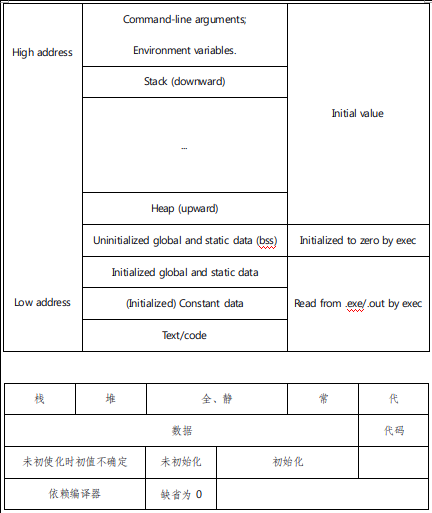
\includegraphics[width=.8\textwidth]{cMemoryLayout2}
  \caption{C Memory Layout}
  \label{fig:c-memory-layout}
\end{figure}

图~\ref{fig:c-memory-layout}~给出了虚拟内存的安排,简洁地说,就两部
分,代码区和数据区。数据区按作用域、生命周期可分堆、栈、常量、全局、
静态。对于全局和静态变量,按是否初始化,分为初始化和未初始化。常量
肯定算作初始化的。其中的 uninitialized data,也即 BSS 表示 ``block
started by symbol''. 总结来看是:\uline{堆,栈,常,代,全、静(初
  始化或未初使化)}。

特别的,图中的最高地址处的命令行参数和环境变量也算作是栈,只不过是
程序在加载时分配,相当于最早入栈的。其中命令行参数部分是传给 main 函数
的 argc 和 argv. 程序运行时还可以指定环境变量,而不是用系统默认的,
如语言编码等。如 \verb|LC=zh_CN.GB18030 ./a.out arg1|.

那么编译后的可执行文件如 a.out (Linux 的 ELF 格式) 或 .exe 是什么样的结构呢?可执行文件
里没有 BSS 段,因为还没有值,只有真正执行时才会有对应的内存。同理
栈、堆也不存在,这三部分只对进程有意义。只有常量,初始化过的全局和
静态变量。不过可执行文件还包含符号表,段表,库链接表,调试等内容。

堆需手动分配、释放,常用 new/delete 和 malloc/free 操作,由低地址往
高地址增长。堆的特点是可根据需求动态分配大小 dynamic allocation on
demand. new/malloc 在堆上分配的内存空间是全局有效的。如果不手
动 delete/free, 则这些分配到的内存在程序执行过程中一直被其占据,直
到程序结束,造成常说的“内存泄露”,导至程序被卡死。所以通常在相同作
用域内申请和释放(如函数内)。

栈是机器自动分配、释放。主要放函数参数,局部变量(自动变量)等。栈上内存主只在
函数局部才有效,函数结束会立即被释放。相反,栈的增长方向是由高往低,
这样是合理的,如果往同一个方向增长,不便于两个区间的管理。

常量区是指存放常量的地方,如:

\begin{lstlisting}
char * p = "hello, world";
printf("%d", 3);
\end{lstlisting}

里 p 是自动变量,分配在栈上。但是字符串 ``hello, world'' 和数字 3
这样的属于量放在常量区。常量区也算作初始化区的一部分。

代码区不用说就是存放放程序代码的地方。

全局变量区是指存放全局变量的地方。静态区是放静态变量的地方。通常这
两个区是合并在一起的。而且这个“全静区”是可以分成未初始化区和已初始化
区两部分。

程序执行时,先把可执行文件(代码,常量,已初始化全、静变量)加载进
内存低地址,再分配未初始化的全、静变量空间。进一步环境变量和程序参
数入栈。后面就是在运行时栈和堆的操作了。

说了这么多,我们来看看 Linux ELF 可执行方件的结构:

\begin{lstlisting}[language=bash,caption={EFL Layout},label={lst:elf-layout}]
  zack@tux ~/workspace/c $ size a.out
   text    data     bss     dec     hex filename
   2391     616      16    3023     bcf a.out
\end{lstlisting}

这里 text 指代码段大小,data 是已初使化全、静变量和常量段大小,bss
段内数据全零。后面的 dec 和 hex 是前面列的和。

\section{数组和链表}

数组和链表都是线性存储结构,但实现方法不同,通常前者在栈上由机器自
动分配,后者在堆上由程序动态分配。实现方法的不同表现出对应的优缺点。

\begin{table}[!htb]
  \centering
  \begin{tabular}{c|c|c}
    \toprule
    \diagbox{优缺点}{结构} & 数组 & 链表 \\
    \midrule
    访问 & 通过下标随机放问 & 要遍历链表顺序查找 \\
    增删 & 慢:要先扩容再移动元素 & 快:只需修改指针指向 \\
    \bottomrule
  \end{tabular}
  \caption{数组和链表}
  \label{tab:array-linkedList}
\end{table}

如果是在中间插入删除(如有序结构),则数组更麻烦,移动的元素更多。

%%% Local Variables:
%%% mode: latex
%%% TeX-master: "main"
%%% End:
